

\chapter{Colinearity}\citep{fox}

Colinearity among predictors is an interesting problem in regression. From one point of view, it is a scourge that reduces the precision of estimates and can make our coefficients unstable. From another point of view, it is the reason we perform multiple regression in the first place. The following offers an explicit example of the problem. Note, however, the actual issue is often less obvious.

I will first describe how it creates problem for precision, as it is an interesting discussion. From there, there really is not much to write about, since most "solutions" are pretty cheap and don't work that well.

\section{Perfect colinearity}

If two predictors in the model are perfectly correlated, they must be measuring the exact same thing. Therefore, it does not make sense to put the same information into the model twice. Don't worry about inadvertently making this mistake, as the {\bf X'X} matrix will not be able to be inverted in this case and your software will produce an error.

\section{Non-perfect colinearity}

This leaves us with the more plausible issue. In any case, two variable in your model are likely to be correlated {\it at least a little bit}. This follows simple logic that if $x$ and $z$ are correlated with $y$, then there must be at least some relationship between $x$ and $z$, even if it is just a little bit.

Again, there is nothing wrong with this, since this is why we want to perform multiple regression in the first place. However, there are limits to how much correlation we can have among our predictors.

\subsection{The variance inflation factor}

Recall from section~\ref{sec:matrixv} that in the bivariate case the variance of the regression coefficient is equation~\eqref{eq:olsb1var}
\[
\mbox{var}\left(\beta_1\right)=\frac{\sigma^2}{\sum_{i=1}^N\left(x_i-\bar{x}\right)^2}
\]
this can be extended to the multiple regression case for slope $j$ of predictor $j$ by adding the variance inflation factor (VIF), $\frac{1}{1-R^2_j}$, to the formula
\begin{equation}\label{eq:olsb1varwvif}
\mbox{var}\left(\beta_j\right)=\frac{1}{1-R^2_j}\frac{\sigma^2}{\left(N-1\right)s^2_j}
\end{equation}
The VIF is literally what it sounds like, its the extent to which (or factor of) the variance of a predictor is increased, given the multiple correlation between it and the other predictors.

Here, $R^2_j$ is the key ingredient. $R^2_j$ is like any other $R^2$ statistic, except here it is how much of predictor $j$ is explained by the {\it other predictors}. The larger $R^2_j$, the larger the variance (and standard error) of $\beta_j$.\footnote{Note, also that since $s^2$ is the variance, we can return to the sum of squares my multiplying the variance by $N-1$.}


\begin{figure}
   \centering
   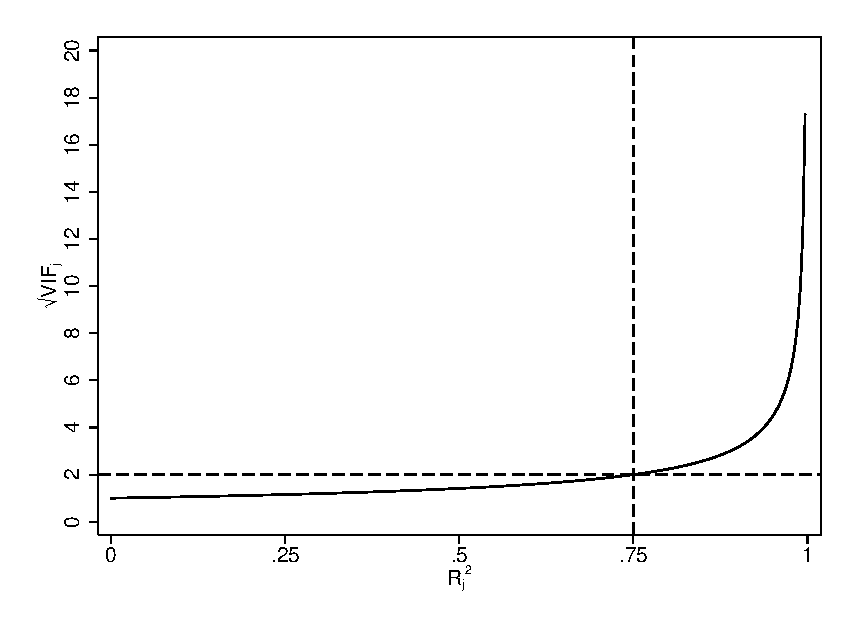
\includegraphics[angle=0,
           width=1\textwidth]{vif.eps}
   \caption{Relationship between the variance inflation factor and $R^2_j$}
  \label{fig:vif}
\end{figure}

But how much is too much correlation among the predictors? Consider Figure~\ref{fig:vif}, where we plot the square root of the VIF against the value of $R^2_j$. Note that the standard error doubles when $R^2_j$ is 0.75. That is, our standard errors only double when three fourths of the variation in one variable is explained by the other predictors. After that, things get worse pretty fast.

\subsection{Example with city data}

The example that follows is pretty silly, but it highlights the issues that you can encounter with high levels of multicolinearity. Suppose the data in Table~\ref{tab:rentdata}, at the end of this chapter. It's census data from the 1980s and includes the average rent, average family income, median household income, and percent of the population with a college degree for various rural places.

Table~\ref{tab:rentcorr} provides the correlations and Figure~\ref{fig:rentmatrix} is a scatter plot matrix of these variables. As you can see, and expectedly, mean family income and median household income are highly correlated.

\begin{table}[htbp]\centering
 \caption{Correlations of variables in Table~\ref{tab:rentdata}
\label{tab:rentcorr}}
\begin{tabular}{lcccc}
\hline
& Mean & Mean family & Median & Percent \\
& rent & income & household & with BA \\
& & & income & \\
\hline
Mean rent & 1.00 \\
Mean family income & 0.63 & 1.00 \\
Median household income & 0.66 & 0.96 & 1.00 \\
Percent with BA & 0.58 & 0.81 & 0.72 & 1.00 \\
\hline
\end{tabular}
\end{table}

An analysis of these data has a simple hypothesis, that higher the family income, holding education constant, the higher rent should be. Now, examine model 1 in Table~\ref{tab:rentmodel}, mean family income has a negative (and significant) slope. This is the other thing that can happen with highly correlated predictors, the sign can flip.

This isn't to say that the model is {\it wrong}, but we have to take it literally: holding the median constant, if the mean increases (i.e. the data become more skewed), rent decreases.

This, however, is not a useful analysis. The better option is to select either the mean family income or the median household income as we do in Models 2 and 3.

The discussion of VIFs can inform the difference in the significance of the effect of education between Model 2 and 3. Notice how, in Table~\ref{tab:rentcorr} that the percent with a college degree is more correlated with mean family income. That correlation is 0.8132, which translates into a VIF of
\[
VIF = \frac{1}{1-R^2_j} = \frac{1}{1-0.8132^2}=2.95
\]
making the effect of education not significant.

However, the correlation with the median income is lower, 0.7238, with a VIF of only 2.10, and the effect of education is now significant.
\[
VIF = \frac{1}{1-R^2_j} = \frac{1}{1-0.7238^2}=2.10
\]

\begin{figure}
   \centering
   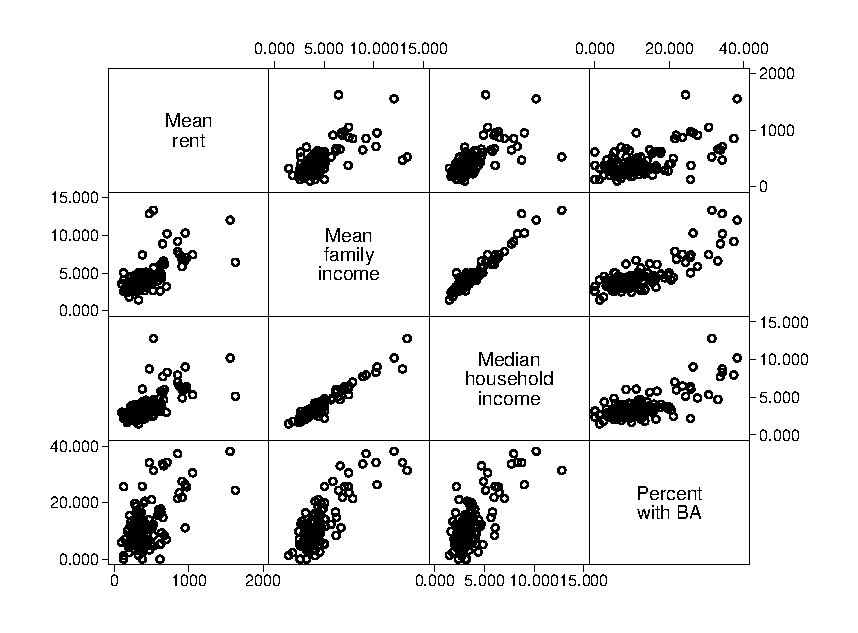
\includegraphics[angle=0,
           width=1\textwidth]{rent_corr.eps}
   \caption{Scatter matrix of variables in Table~\ref{tab:rentdata}}
  \label{fig:rentmatrix}
\end{figure}

\begin{table}[htbp]\centering
 \caption{Models predicting mean rent in census places Table~\ref{tab:rentdata}
\label{tab:rentmodel}}
\begin{tabular}{lccc}
\hline
Variable      &    Model 1 & Model 2 & Model 3 \\
\hline
Mean family income  &   -79.636* &   56.360***&        \\
      &  (38.517)  &  (14.952)  &        \\
Median household income  &   140.822***&        &   69.508***\\
      &  (37.090)  &        &  (13.827)  \\
Percent with BA  &   0.111** &    0.060  &    0.064* \\
      &   (0.037)  &   (0.036)  &   (0.029)  \\
Intercept  &   133.748** &   106.433* &   96.588* \\
      &  (43.034)  &  (44.795)  &  (39.645)  \\
\hline
\multicolumn{4}{l}{Model Statistics} \\
\hline
N      &   120.000  &   120.000  &   120.000  \\
F      &   34.683  &   40.206  &   48.528  \\
$R^2$    &    0.473  &    0.407  &    0.453  \\
$df$ Regression     &    3.000  &    2.000  &    2.000  \\
Sum of Squares Regression     & 3548574.288  & 3056921.326  & 3402777.993  \\
$df$ Error     &   116.000  &   117.000  &   117.000  \\
Sum of Squares Error     & 3956217.179  & 4447870.140  & 4102013.473  \\
\hline
\multicolumn{4}{l}{Variance Inflation Factors} \\
\hline
Mean Income & 21.81 & 2.95 & \\
Median Income & 15.55 & & 2.10 \\
Percent with BA & 3.40 & 2.95 & 2.10 \\
\hline
\multicolumn{4}{l}{$SE$s in parentheses, $*p<0.05,**p<0.01,***p<0.001$} \\
\hline
\end{tabular}
\end{table}

\subsection{What to do?}
There are essentially two things you can do to solve colinearity:
\begin{itemize}
\item{drop variables}
\item{combine variables}
\end{itemize}

\subsubsection{Drop variables}
This is essentially what we did in Models 2 and 3 in Table~\ref{tab:rentmodel}. Since we can make the argument that both income variables are essentially measuring the same thing, we just pick one and be done with it.

\subsubsection{Combine variables}
The other option is to use factor analysis (which is beyond the scope of these notes for now) to create a common factor score that combines the information from the predictors which are highly correlated.

\section*{For more information}
For treatment of multicollinearity in regression, see \citep{fox} and \citep{hill}. For comprehensive regression analysis, consult \citep{agresti} and \citep{cameron2005microeconometrics}.